% ==============================================================
% Section 3: System Overview
% ==============================================================
\section{System Overview}

\begin{frame}{System Overview: L\_RAG at a Glance}
\small
\centering
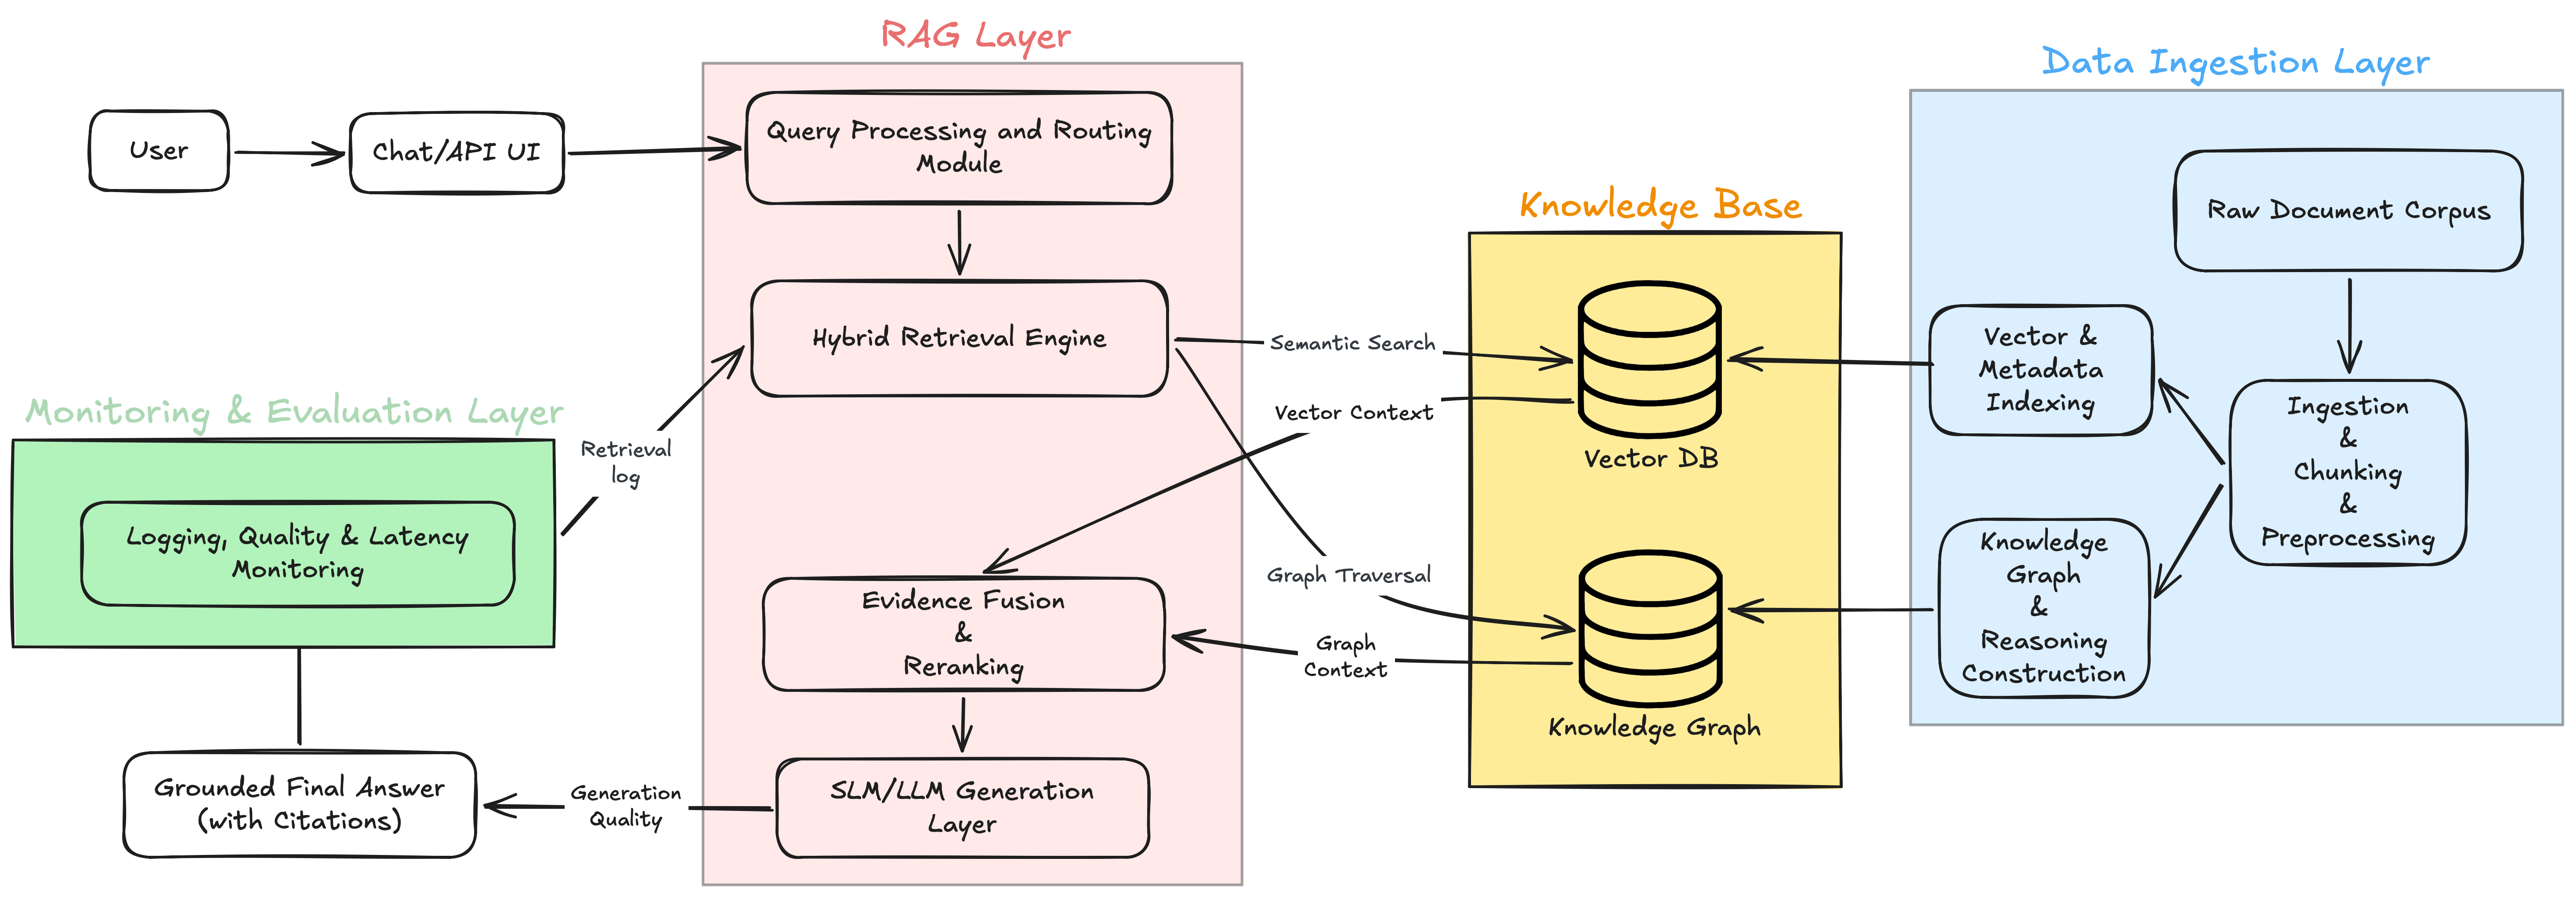
\includegraphics[width=0.96\linewidth]{imgs/system_architecture.png}
\vspace{0.01cm}

\begin{block}{End-to-End Visual Architecture}
\centering
\scriptsize
Hybrid Dense-Sparse Search $\parallel$ Knowledge Graph Overlay $\parallel$ Sequential Reranking $\parallel$ Citation-Grounded LLM
\end{block}

\end{frame}

\begin{frame}{L\_RAG Pipeline: Stage-by-Stage Processing}
\scriptsize
\begin{columns}[T]
  \column{0.48\textwidth}
    \begin{block}{Stage 1: Indexing \& Representation}
    \begin{itemize}
      \item \textbf{Dense E5:} Metadata enrichment (\texttt{Title $\parallel$ Header $\parallel$ Passage}) stored in FAISS \texttt{IndexFlatIP}.
      \item \textbf{Sparse BM25:} \texttt{underthesea} tokenizer preserves compound legal terms (\texttt{trach\_nhiem\_hinh\_su}).
    \end{itemize}
    \end{block}

    \begin{block}{Stage 2: KG Overlay Joiner}
    \begin{itemize}
      \item \textbf{Validity Masking:} Dynamic \texttt{id\_str\_filter} excludes superseded provisions by \texttt{as\_of\_date}.
      \item \textbf{1-Hop Expansion:} Traverses \texttt{CHUNK\_NEXT} pointers to retrieve sibling context.
    \end{itemize}
    \end{block}

  \column{0.48\textwidth}
    \begin{block}{Stage 3: Fusion \& Sequential Reranking}
    \begin{itemize}
      \item \textbf{RRF Fusion ($k=60$):} Merges Dense \& BM25 hits into candidate pool $C_{30}$.
      \item \textbf{Cross-Encoder Reranking:} Sequential GPU load-run-unload cycle yields Top $N=10$ chunks.
    \end{itemize}
    \end{block}

    \begin{block}{Stage 4: Grounded LLM Generation}
    \begin{itemize}
      \item \textbf{Model:} \texttt{gpt-4o-mini} ($T=0.0$, Max tokens 1024).
      \item \textbf{Guardrails:} Strict statutory citation grounding + \texttt{INSUFFICIENT\_CONTEXT} abstention.
    \end{itemize}
    \end{block}
\end{columns}
\end{frame}

\begin{frame}{G-LRAG Knowledge Graph: Schema \& Construction}
\small
\begin{columns}[T]
  \column{0.52\textwidth}
    \begin{block}{Graph Node Hierarchy}
    \scriptsize
    \begin{itemize}
      \item \textbf{Documents ($D$):} Title, Authority rank, Issuing body, Effective date, Validity status.
      \item \textbf{Provisions ($P$):} Article/Clause header, Statutory type.
      \item \textbf{Chunks ($C$):} Passage text, Sequence ID.
    \end{itemize}
    \end{block}

    \begin{block}{Edge Relationships}
    \scriptsize
    \begin{itemize}
      \item \textbf{Structural Edges:} \texttt{DOC\_HAS\_PROVISION}, \texttt{PROVISION\_HAS\_CHUNK}, \texttt{CHUNK\_NEXT}, \texttt{PROVISION\_NEXT}.
      \item \textbf{Legal Relations:} Amend, Replace, Cite, Repeal between legal instruments.
    \end{itemize}
    \end{block}

  \column{0.45\textwidth}
    \begin{block}{Ingested Corpus Scale}
    \scriptsize
    \centering
    \begin{tabular}{lr}
    \toprule
    \textbf{Entity Type} & \textbf{Total Count} \\
    \midrule
    \textbf{Documents} & 151,624 \\
    \textbf{Provisions} & 1,386,267 \\
    \textbf{Chunks} & 1,513,376 \\
    \textbf{Document Edges} & 883,256 \\
    \textbf{External Stubs} & 19,763 \\
    \bottomrule
    \end{tabular}
    \end{block}

    \begin{alertblock}{Construction Rule}
    \scriptsize
    Draft/unverified records quarantined; dynamic validity whitelisting by \texttt{as\_of\_date}.
    \end{alertblock}
\end{columns}
\end{frame}


